\documentclass[12pt,letterpaper]{article}
\usepackage{graphicx,textcomp}
\usepackage{natbib}
\usepackage{setspace}
\usepackage{fullpage}
\usepackage{color}
\usepackage[reqno]{amsmath}
\usepackage{amsthm}
\usepackage{fancyvrb}
\usepackage{amssymb,enumerate}
\usepackage[all]{xy}
\usepackage{endnotes}
\usepackage{lscape}
\newtheorem{com}{Comment}
\usepackage{float}
\usepackage{hyperref}
\newtheorem{lem} {Lemma}
\newtheorem{prop}{Proposition}
\newtheorem{thm}{Theorem}
\newtheorem{defn}{Definition}
\newtheorem{cor}{Corollary}
\newtheorem{obs}{Observation}
\usepackage[compact]{titlesec}
\usepackage{dcolumn}
\usepackage{tikz}
\usetikzlibrary{arrows}
\usepackage{multirow}
\usepackage{xcolor}
\newcolumntype{.}{D{.}{.}{-1}}
\newcolumntype{d}[1]{D{.}{.}{#1}}
\definecolor{light-gray}{gray}{0.65}
\usepackage{url}
\usepackage{listings}
\usepackage{color}


\definecolor{codegreen}{rgb}{0,0.6,0}
\definecolor{codegray}{rgb}{0.5,0.5,0.5}
\definecolor{codepurple}{rgb}{0.58,0,0.82}
\definecolor{backcolour}{rgb}{0.95,0.95,0.92}

\lstdefinestyle{mystyle}{
	backgroundcolor=\color{backcolour},   
	commentstyle=\color{codegreen},
	keywordstyle=\color{magenta},
	numberstyle=\tiny\color{codegray},
	stringstyle=\color{codepurple},
	basicstyle=\footnotesize,
	breakatwhitespace=false,         
	breaklines=true,                 
	captionpos=b,                    
	keepspaces=true,                 
	numbers=left,                    
	numbersep=5pt,                  
	showspaces=false,                
	showstringspaces=false,
	showtabs=false,                  
	tabsize=2
}
\lstset{style=mystyle}
\newcommand{\Sref}[1]{Section~\ref{#1}}
\newtheorem{hyp}{Hypothesis}

\title{Problem Set 1}
\date{Due: October 9, 2025}
\author{Applied Stats/Quant Methods 1}

\begin{document}
	\maketitle
	
	\section*{Instructions}
	\begin{itemize}
	\item Please show your work! You may lose points by simply writing in the answer. If the problem requires you to execute commands in \texttt{R}, please include the code you used to get your answers. Please also include the \texttt{.R} file that contains your code. If you are not sure if work needs to be shown for a particular problem, please ask.
\item Your homework should be submitted electronically on GitHub.
\item This problem set is due before 23:59 on Thursday October 9, 2025. No late assignments will be accepted.
	\end{itemize}
	
	\vspace{1cm}
	\section*{Question 1: Education}

A school counselor was curious about the average of IQ of the students in her school and took a random sample of 25 students' IQ scores. The following is the data set:\\
\vspace{.5cm}

\lstinputlisting[language=R, firstline=36, lastline=36]{PS01.R}  

\vspace{1cm}

\begin{enumerate}
	\item Find a 90\% confidence interval for the average student IQ in the school.\\

\newpage

\textbf{Finding a 90\% confidence interval}

\noindent \underline{Step 1}: Calculate the sample mean. The sample mean equals the sum of the values divided by the number of values in the sample (n).

\lstinputlisting[language=R, firstline=52, lastline=56]{PS01_answers_KC.R}
\begin{verbatim}
[1] 98.44
\end{verbatim}

\noindent \underline{Step 2}: Calculate the standard deviation 

\noindent Find how much each data point differs from the mean and square each value. 

\lstinputlisting[language=R, firstline=60, lastline=62]{PS01_answers_KC.R}

\noindent Add the squared values to find the sum of squares
\lstinputlisting[language=R, firstline=65, lastline=65]{PS01_answers_KC.R}

\noindent Find the variance by dividing the sum of squared by the degrees of freedom (the number of values in a sample (n) minus 1)

\lstinputlisting[language=R, firstline=69, lastline=69]{PS01_answers_KC.R}  

\noindent Find the standard deviation (the square root of variance)

\lstinputlisting[language=R, firstline=72, lastline=73]{PS01_answers_KC.R}

\begin{verbatim}
[1] 13.09287
\end{verbatim}

\noindent \underline{Step 3}: Calculate the standard error, which equals the standard deviation divided by the square root of n(the number of observations in the sample)

\lstinputlisting[language=R, firstline=78, lastline=79]{PS01_answers_KC.R}  

\begin{verbatim}
[1] 2.618575
\end{verbatim}

\newpage

\noindent \underline{Step 4}: Calculate the t-score by inputting in R: 
	\begin{itemize}
\item (1 minus the confidence coefficient) divided by 2. Since we are finding a 90\% confidence interval, the confidence coefficient is 0.9, and 1 - 0.9 = 0.1. 
\item The degrees of freedom (n-1)
    \end{itemize}
    
\lstinputlisting[language=R, firstline=85, lastline=86]{PS01_answers_KC.R}  

\begin{verbatim}
[1] -1.710882
\end{verbatim}

\noindent \underline{Step 6}: Calculate the lower limit of the confidence interval by calculating the sample mean - (the absolute value of the t-score * standard error)

\lstinputlisting[language=R, firstline=91, lastline=92]{PS01_answers_KC.R}

\begin{verbatim}
[1] 93.95993
\end{verbatim}

\noindent \underline{Step 7}: Calculate the upper limit of the confidence interval by calculating the sample mean + (the absolute value of the t-score * standard error)

\lstinputlisting[language=R, firstline=97, lastline=98]{PS01_answers_KC.R}

\begin{verbatim}
[1] 102.9201
\end{verbatim}

\noindent \textbf{Conclusion}: Based on the confidence interval, we are 90 percent confident that the true mean of IQ at the school is between 93.95993 and 102.9201.

\newpage

\item Next, the school counselor was curious  whether  the average student IQ in her school is higher than the average IQ score (100) among all the schools in the country.\\ 
	
\noindent Using the same sample, conduct the appropriate hypothesis test with $\alpha=0.05$.

\vspace{.5cm}

\textbf{Conducting a hypothesis test}

\noindent \underline{Step 1}: Assumptions

	\begin{itemize}
	\item Due to the fact that n is less than 30, we cannot assume a normal distribution. So, I will perform a t-test instead of a z-test
	
	\item The data is continuous
	
	\item The sample was random
	\end{itemize}

\noindent \underline{Step 2}: State Hypotheses

	\begin{itemize}
\item Alternative Hypothesis: The average student IQ in the school counselor's school is greater than 100

\item Null Hypothesis: The average student IQ in the school counselor's school is less than or equal to 100 
	\end{itemize}
	
\noindent \underline{Step 3}: Calculate the test statistic (sample mean - population mean)/(sample SE)\\

\lstinputlisting[language=R, firstline=119, lastline=120]{PS01_answers_KC.R}

\begin{verbatim}
[1] -0.5957439
\end{verbatim}

\noindent \underline{Step 4}: Calculate the p-value by inputting the test statistic and the degrees of freedom (sample size - 1). lower.tail = FALSE was used because it is a one-sided hypothesis test in which we are examining the upper tail of the curve.

\lstinputlisting[language=R, firstline=122, lastline=122]{PS01_answers_KC.R}

\begin{verbatim}
[1] 0.7215383
\end{verbatim}

\noindent \textbf{Conclusion}: The calculated p-value is greater than the critical value of 0.05.\break Therefore, we fail to reject the null hypothesis that the average student IQ in the school counselor's school is less than or equal to 100.

\end{enumerate}

\newpage

	\section*{Question 2: Political Economy}

\noindent Researchers are curious about what affects the amount of money communities spend on addressing homelessness. The following variables constitute our data set about social welfare expenditures in the USA. \\
\vspace{.5cm}


\begin{tabular}{r|l}
	\texttt{State} &\emph{50 states in US} \\
	\texttt{Y} & \emph{per capita expenditure on shelters/housing assistance in state}\\
	\texttt{X1} &\emph{per capita personal income in state} \\
	\texttt{X2} &  \emph{Number of residents per 100,000 that are "financially insecure" in state}\\
	\texttt{X3} &  \emph{Number of people per thousand residing in urban areas in state} \\
	\texttt{Region} &  \emph{1=Northeast, 2= North Central, 3= South, 4=West} \\
\end{tabular}

\vspace{.5cm}
\noindent Explore the \texttt{expenditure} data set and import data into \texttt{R}.
\vspace{.5cm}
\lstinputlisting[language=R, firstline=54, lastline=54]{PS01.R}  
\vspace{.5cm}
\begin{itemize}

\item
Please plot the relationships among \emph{Y}, \emph{X1}, \emph{X2}, and \emph{X3}? What are the correlations among them (you just need to describe the graph and the relationships among them)?

\vspace{.5cm}
\item
Please plot the relationship between \emph{Y} and \emph{Region}? On average, which region has the highest per capita expenditure on housing assistance?
\vspace{.5cm}
\item
Please plot the relationship between \emph{Y} and \emph{X1}? Describe this graph and the relationship. Reproduce the above graph including one more variable \emph{Region} and display different regions with different types of symbols and colors.

\newpage

\noindent \textbf{Plotting the relationships among Y, X1, X2, and X3}

\lstinputlisting[language=R, firstline=144, lastline=144]{PS01_answers_KC.R}

\begin{figure}[!ht]
	\caption{Plot of Y, X1, X2, and X3}
	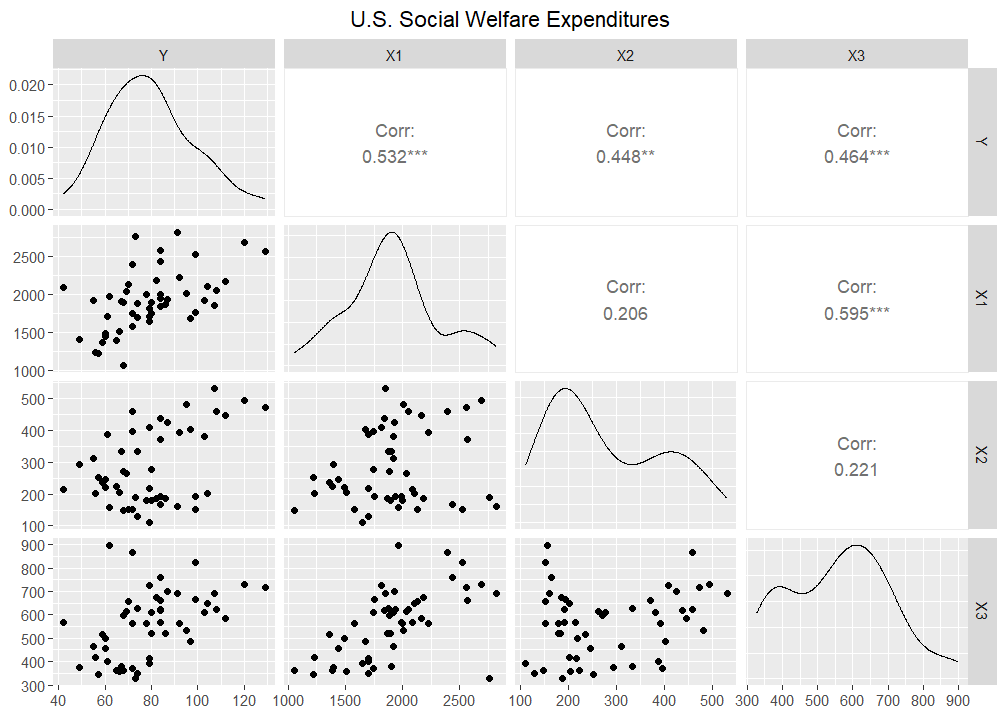
\includegraphics[width=\textwidth]{US_Social_Welfare_Expenditures.png}
\end{figure}

\item Per capita personal income in state (X1) and per capita expenditure on shelters/housing assistance in state (Y) are positively correlated. The form appears relatively linear, moderately spread out, and somewhat strong. A correlation coefficient of 0.532 indicates that it is a moderate positive correlation.

\item Per capita expenditure on shelters/housing assistance in state (Y) is positively correlated with number of residents per 100,000 that are ”financially insecure” in state (X2). The correlation appears relatively strong as the points are somewhat close together. The form appears to curve, indicating that a linear measurement may not be the best way of analyzing this data. A correlation coefficient of 0.448 indicates a moderate positive linear correlation.

\newpage

\item Per capita personal income in state (X1) is positively correlated with the number of residents per 100,000 that are ”financially insecure” in state (X2). The form is relatively spread out, and the strength appears rather weak. A correlation coefficient of 0.206 suggests there is a weak/negligible correlation.

\item Per capita expenditure on shelters/housing assistance in state (Y) is positively correlated with the number of people per thousand residing in urban areas in state (X3). The form appears relatively linear and the data points are moderately close together. A correlation coefficient of 0.464 suggests a moderate positive correlation.

\item Per capita personal income in state (X1) is positively correlated with the number of people per thousand residing in urban areas in state (X3). The distribution appears relatively linear and moderately clustered together. A correlation coefficient of 0.595 indicates a moderate positive association. This is the largest correlation coefficient and the tightest grouping that we see among variables in this data set.

\item The number of residents per 100,000 that are ”financially insecure” in state (X2) and the number of people per thousand residing in urban areas in state (X3) are positively correlated. The distribution appears very spread out and there is no apparent pattern. A correlation coefficient of 0.221 indicates a weak/negligible positive correlation.
\end{itemize}
\newpage

\noindent \textbf{Plotting the relationship between Y and Region}

\lstinputlisting[language=R, firstline=177, lastline=182]{PS01_answers_KC.R}

\begin{figure}[!h]
	\caption{Plot of Y and Region}
	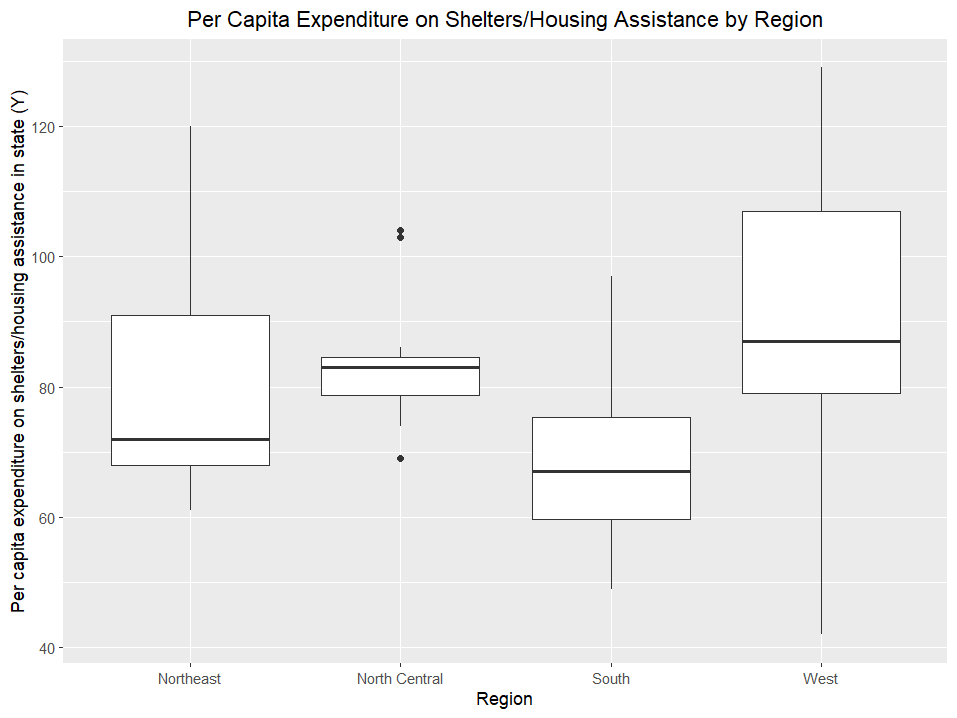
\includegraphics[width=\textwidth]{Expenditure_By_Region.png}
\end{figure}

\noindent On average, the West has the highest per capita expenditure on housing assistance. The North Central region has the next highest average housing assistance expenditure, followed by the Northeast. Lastly, the South has the lowest average per capita expenditure on housing assistance.

\newpage

\noindent \textbf{Plotting the relationship between Y and X1}

\lstinputlisting[language=R, firstline=190, lastline=194]{PS01_answers_KC.R}

\begin{figure}[!h]
	\caption{Plot of Y and X1}
	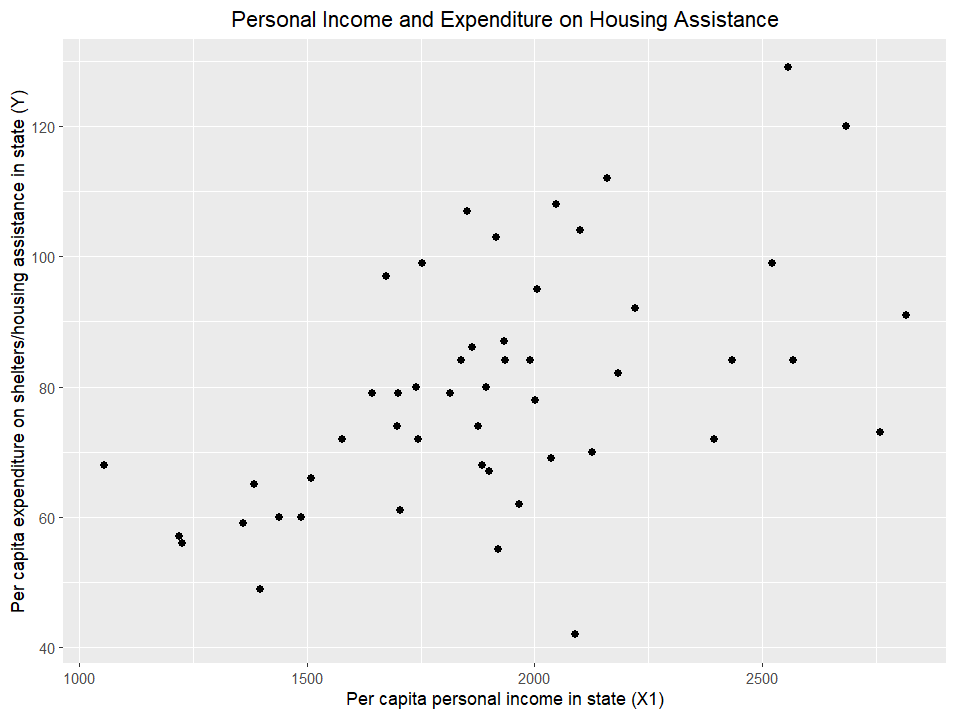
\includegraphics[width=\textwidth]{Expenditure_By_Income.png}
\end{figure}

\noindent This graph appears to demonstrate a positive, moderately strong, and relatively linear correlation between per capita personal income in state (X1) and per capita expenditure on shelters/housing assistance in state (Y)

\newpage

\lstinputlisting[language=R, firstline=198, lastline=204]{PS01_answers_KC.R}

\begin{figure}[!h]
	\caption{Plot of Y, X1, and Region}
	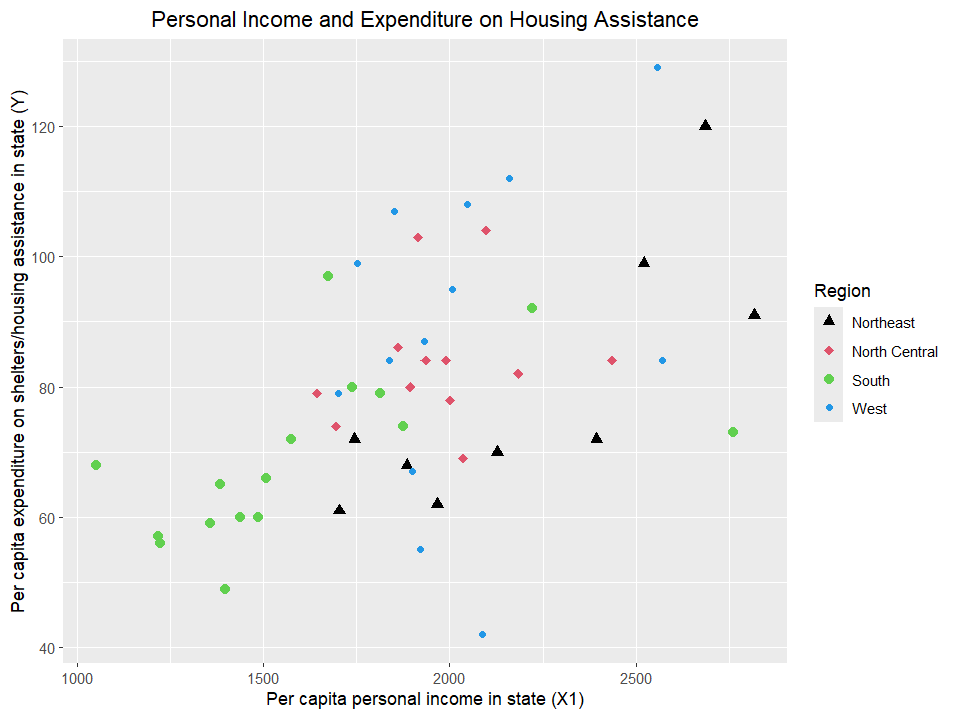
\includegraphics[width=\textwidth]{Expenditure_By_Income_With_Region.png}
\end{figure}

\noindent This graph suggests that the positive linear correlation between per capita personal income in state and per capita expenditure on housing in state may have region as a confounding variable. Some regional data points are clustered together. In particular, the South has a grouping of points that have both low per capita personal income in state and low expenditure on shelter/housing assistance. This example highlights the danger of assuming a causal relationship based on correlation, as this graph reveals a more complex relationship between the variables than it appeared from the graph of just X1 and Y.

\end{document}
